\documentclass[11pt,a4paper,]{article}
\usepackage{lmodern}

\usepackage{amssymb,amsmath}
\usepackage{ifxetex,ifluatex}
\usepackage{fixltx2e} % provides \textsubscript
\ifnum 0\ifxetex 1\fi\ifluatex 1\fi=0 % if pdftex
  \usepackage[T1]{fontenc}
  \usepackage[utf8]{inputenc}
\else % if luatex or xelatex
  \usepackage{unicode-math}
  \defaultfontfeatures{Ligatures=TeX,Scale=MatchLowercase}
\fi
% use upquote if available, for straight quotes in verbatim environments
\IfFileExists{upquote.sty}{\usepackage{upquote}}{}
% use microtype if available
\IfFileExists{microtype.sty}{%
\usepackage[]{microtype}
\UseMicrotypeSet[protrusion]{basicmath} % disable protrusion for tt fonts
}{}
\PassOptionsToPackage{hyphens}{url} % url is loaded by hyperref
\usepackage[unicode=true]{hyperref}
\hypersetup{
            pdftitle={Zomato - Best of Melbourne Analysis},
            pdfborder={0 0 0},
            breaklinks=true}
\urlstyle{same}  % don't use monospace font for urls
\usepackage{geometry}
\geometry{a4paper, centering, text={16cm,24cm}}
\usepackage[style=authoryear-comp,]{biblatex}
\addbibresource{references.bib}
\usepackage{longtable,booktabs}
% Fix footnotes in tables (requires footnote package)
\IfFileExists{footnote.sty}{\usepackage{footnote}\makesavenoteenv{long table}}{}
\usepackage{graphicx,grffile}
\makeatletter
\def\maxwidth{\ifdim\Gin@nat@width>\linewidth\linewidth\else\Gin@nat@width\fi}
\def\maxheight{\ifdim\Gin@nat@height>\textheight\textheight\else\Gin@nat@height\fi}
\makeatother
% Scale images if necessary, so that they will not overflow the page
% margins by default, and it is still possible to overwrite the defaults
% using explicit options in \includegraphics[width, height, ...]{}
\setkeys{Gin}{width=\maxwidth,height=\maxheight,keepaspectratio}
\IfFileExists{parskip.sty}{%
\usepackage{parskip}
}{% else
\setlength{\parindent}{0pt}
\setlength{\parskip}{6pt plus 2pt minus 1pt}
}
\setlength{\emergencystretch}{3em}  % prevent overfull lines
\providecommand{\tightlist}{%
  \setlength{\itemsep}{0pt}\setlength{\parskip}{0pt}}
\setcounter{secnumdepth}{5}

% set default figure placement to htbp
\makeatletter
\def\fps@figure{htbp}
\makeatother


\title{Zomato - Best of Melbourne Analysis}

%% MONASH STUFF

%% CAPTIONS
\RequirePackage{caption}
\DeclareCaptionStyle{italic}[justification=centering]
 {labelfont={bf},textfont={it},labelsep=colon}
\captionsetup[figure]{style=italic,format=hang,singlelinecheck=true}
\captionsetup[table]{style=italic,format=hang,singlelinecheck=true}


%% FONT
\RequirePackage{bera}
\RequirePackage[charter,expert,sfscaled]{mathdesign}
\RequirePackage{fontawesome}

%% HEADERS AND FOOTERS
\RequirePackage{fancyhdr}
\pagestyle{fancy}
\rfoot{\Large\sffamily\raisebox{-0.1cm}{\textbf{\thepage}}}
\makeatletter
\lhead{\textsf{\expandafter{\@title}}}
\makeatother
\rhead{}
\cfoot{}
\setlength{\headheight}{15pt}
\renewcommand{\headrulewidth}{0.4pt}
\renewcommand{\footrulewidth}{0.4pt}
\fancypagestyle{plain}{%
\fancyhf{} % clear all header and footer fields
\fancyfoot[C]{\sffamily\thepage} % except the center
\renewcommand{\headrulewidth}{0pt}
\renewcommand{\footrulewidth}{0pt}}

%% MATHS
\RequirePackage{bm,amsmath}
\allowdisplaybreaks

%% GRAPHICS
\RequirePackage{graphicx}
\setcounter{topnumber}{2}
\setcounter{bottomnumber}{2}
\setcounter{totalnumber}{4}
\renewcommand{\topfraction}{0.85}
\renewcommand{\bottomfraction}{0.85}
\renewcommand{\textfraction}{0.15}
\renewcommand{\floatpagefraction}{0.8}


%\RequirePackage[section]{placeins}

%% SECTION TITLES


%% SECTION TITLES (NEW: Changing sections and subsections color)  
\RequirePackage[compact,sf,bf]{titlesec}
\titleformat*{\section}{\Large\sf\bfseries\color[rgb]{0.8, 0.7, 0.1 }}
\titleformat*{\subsection}{\large\sf\bfseries\color[rgb]{0.8, 0.7, 0.1 }}
\titleformat*{\subsubsection}{\sf\bfseries\color[rgb]{0.8, 0.7, 0.1 }}
\titlespacing{\section}{0pt}{2ex}{.5ex}
\titlespacing{\subsection}{0pt}{1.5ex}{0ex}
\titlespacing{\subsubsection}{0pt}{.5ex}{0ex}


%% TITLE PAGE
\def\Date{\number\day}
\def\Month{\ifcase\month\or
 January\or February\or March\or April\or May\or June\or
 July\or August\or September\or October\or November\or December\fi}
\def\Year{\number\year}

%% LINE AND PAGE BREAKING
\sloppy
\clubpenalty = 10000
\widowpenalty = 10000
\brokenpenalty = 10000
\RequirePackage{microtype}

%% PARAGRAPH BREAKS
\setlength{\parskip}{1.4ex}
\setlength{\parindent}{0em}

%% HYPERLINKS
\RequirePackage{xcolor} % Needed for links
\definecolor{darkblue}{rgb}{0,0,.6}
\RequirePackage{url}

\makeatletter
\@ifpackageloaded{hyperref}{}{\RequirePackage{hyperref}}
\makeatother
\hypersetup{
     citecolor=0 0 0,
     breaklinks=true,
     bookmarksopen=true,
     bookmarksnumbered=true,
     linkcolor=darkblue,
     urlcolor=blue,
     citecolor=darkblue,
     colorlinks=true}

\usepackage[showonlyrefs]{mathtools}
\usepackage[no-weekday]{eukdate}

%% BIBLIOGRAPHY   %------------------------------------------------------------------------------------------------

\makeatletter
\@ifpackageloaded{biblatex}{}{\usepackage[style=authoryear-comp, backend=biber, natbib=true]{biblatex}}
\makeatother
\ExecuteBibliographyOptions{bibencoding=utf8,minnames=1,maxnames=3, maxbibnames=99,dashed=false,terseinits=true,giveninits=true,uniquename=false,uniquelist=false,doi=false, isbn=false,url=true,sortcites=false}

\DeclareFieldFormat{url}{\texttt{\url{#1}}}
\DeclareFieldFormat[article]{pages}{#1}
\DeclareFieldFormat[inproceedings]{pages}{\lowercase{pp.}#1}
\DeclareFieldFormat[incollection]{pages}{\lowercase{pp.}#1}
\DeclareFieldFormat[article]{volume}{\mkbibbold{#1}}
\DeclareFieldFormat[article]{number}{\mkbibparens{#1}}
\DeclareFieldFormat[article]{title}{\MakeCapital{#1}}
\DeclareFieldFormat[article]{url}{}
%\DeclareFieldFormat[book]{url}{}
%\DeclareFieldFormat[inbook]{url}{}
%\DeclareFieldFormat[incollection]{url}{}
%\DeclareFieldFormat[inproceedings]{url}{}
\DeclareFieldFormat[inproceedings]{title}{#1}
\DeclareFieldFormat{shorthandwidth}{#1}
%\DeclareFieldFormat{extrayear}{}
% No dot before number of articles
\usepackage{xpatch}
\xpatchbibmacro{volume+number+eid}{\setunit*{\adddot}}{}{}{}
% Remove In: for an article.
\renewbibmacro{in:}{%
  \ifentrytype{article}{}{%
  \printtext{\bibstring{in}\intitlepunct}}}

\AtEveryBibitem{\clearfield{month}}
\AtEveryCitekey{\clearfield{month}}

\makeatletter
\DeclareDelimFormat[cbx@textcite]{nameyeardelim}{\addspace}
\makeatother

\author{\sf\Large\textbf{ Dea Avega Editya}\\ {\sf\large Master of BA\\[0.5cm]} \sf\Large\textbf{ Muhammad Soban Qasim}\\ {\sf\large Master of BA\\[0.5cm]} \sf\Large\textbf{ Abhishek Sinha}\\ {\sf\large Master of BA\\[0.5cm]} \sf\Large\textbf{ Vinny Vu}\\ {\sf\large Master of BA\\[0.5cm]}}

\date{\sf\Date~\Month~\Year}
\makeatletter
\lfoot{\sf Editya, Qasim, Sinha, Vu: \@date}
\makeatother


%%%% PAGE STYLE FOR FRONT PAGE OF REPORTS    %----------------------------------------------------------------------------------------

\makeatletter
\def\organization#1{\gdef\@organization{#1}}
\def\telephone#1{\gdef\@telephone{#1}}
\def\email#1{\gdef\@email{#1}}
\makeatother
  \organization{ETC5513 Collaborative and Reproductible Practices}

  \def\name{Our consultancy \newline add names \&\newline add names}

  \telephone{(03) 9905 2478}

  \email{questions@company.com}                 %NEW: New email addresss ---------------------------------------

\def\webaddress{\url{http://company.com/stats/consulting/}} %NEW: URl  ------------------------------------------
\def\abn{12 377 614 630}                                    % NEW: ABN -------------------------------------------  
\def\logo{\includegraphics[width=6cm]{logo}}  %NEW: Changing logo
\def\extraspace{\vspace*{1.6cm}}
\makeatletter
\def\contactdetails{\faicon{phone} & \@telephone \\
                    \faicon{envelope} & \@email}
\makeatother

%%%% FRONT PAGE OF REPORTS

\def\reporttype{Report for}

\long\def\front#1#2#3{
\newpage
\begin{singlespacing}
\thispagestyle{empty}
\vspace*{-1.4cm}
\hspace*{-1.4cm}
\hbox to 16cm{
  \hbox to 6.5cm{\vbox to 14cm{\vbox to 25cm{
    \logo
    \vfill
    \parbox{6.3cm}{\raggedright
      \sf\color[rgb]{0, 0.29, 0.55}    % NEW color -company info------------------------------------------------------------------------------------
      {\large\textbf{\name}}\par
      \vspace{.7cm}
      \tabcolsep=0.12cm\sf\small
      \begin{tabular}{@{}ll@{}}\contactdetails
      \end{tabular}
      \vspace*{0.3cm}\par
      ABN: \abn\par
    }
  }\vss}\hss}
  \hspace*{0.2cm}
  \hbox to 1cm{\vbox to 14cm{\rule{4pt}{26.8cm}\vss}\hss\hfill}  %NEW: Thicker vertical line -----------------------------------------------------
  \hbox to 10cm{\vbox to 14cm{\vbox to 25cm{   
      \vspace*{3cm}\sf\raggedright
      \parbox{11cm}{\sf\raggedright\baselineskip=1.2cm
         \fontsize{24.88}{30}\color[rgb]{0, 0.29, 0.55}\sf\textbf{#1}}   % NEW: title color blue ----------------------------------------------
      \par
      \vfill
      \large
      \vbox{\parskip=0.8cm #2}\par
      \vspace*{2cm}\par
      \reporttype\\[0.3cm]
      \hbox{#3}%\\[2cm]\
      \vspace*{1cm}
      {\large\sf\textbf{\Date~\Month~\Year}}
   }\vss}
  }}
\end{singlespacing}
\newpage
}

\makeatletter
\def\titlepage{\front{\expandafter{\@title}}{\@author}{\@organization}}
\makeatother

\usepackage{setspace}
\setstretch{1.5}

%% Any special functions or other packages can be loaded here.

\usepackage{float}
\let\origfigure\figure
\let\endorigfigure\endfigure
\renewenvironment{figure}[1][2] {
    \expandafter\origfigure\expandafter[H]
} {
    \endorigfigure
}%% Any special functions or other packages can be loaded here.
\usepackage{booktabs}
\usepackage{longtable}
\usepackage{array}
\usepackage{multirow}
\usepackage{wrapfig}
\usepackage{float}
\usepackage{colortbl}
\usepackage{pdflscape}
\usepackage{tabu}
\usepackage{threeparttable}
\usepackage{threeparttablex}
\usepackage[normalem]{ulem}
\usepackage{makecell}


\begin{document}           % Begining of document body -----------------------------------------------
\titlepage

{
\setcounter{tocdepth}{2}
\tableofcontents
}
\clearpage

\section*{Introduction}

\hypertarget{git-repository}{%
\section{Git Repository}\label{git-repository}}

Access the git repository for this project via the following \href{https://github.com/dedi0003/assignment4_etc5513}{link}

\hypertarget{introduction}{%
\section{Introduction}\label{introduction}}

For this assignment we will be looking at scrapping data from Zomato, one of the largest foods aggregators in the world \textcite{zomato}. Zomato provides information on restaurants including, price, location, reviews and more. For the purposes on our analysis we will be looking at the best of Melbourne list \textcite{zomatomelb} to gain insight into some of the most popular restaurants in Melbourne.

This report will include four sections looking at:

\begin{itemize}
\tightlist
\item
  Is expensive food better than cheap food?
\item
  Finding the very best restaurants in Melbourne
\item
  Popularity of different cuisine in Melbourne
\item
  Exploring restaurants with gluten free food in Melbourne
\end{itemize}

In this report we have used the following packages \textcite{tidyverse}, \textcite{romato}, \textcite{kableExtra}, \textcite{knitr}, \textcite{dplyr}, \textcite{ggplot2}, \textcite{leaflet}, \textcite{readr}, \textcite{mapview}, \textcite{viridis}, \textcite{plotly}.

\clearpage

\hypertarget{is-expensive-food-better-than-cheap-food}{%
\section{Is expensive food better than cheap food?}\label{is-expensive-food-better-than-cheap-food}}

In this section we will be using the Zomato Best of Melbourne to explore whether expensive food is ``better'' than cheap food. To conduct this analysis, we will be looking at:

\begin{itemize}
\tightlist
\item
  What is considered cheap and expensive food
\item
  What the breakdown of price ranges of the restaurants is
\item
  Comparing prices and aggregate ratings
\item
  Determining whether there is a relationship between prices and ratings
\end{itemize}

\hypertarget{what-is-considered-cheap-and-expensive-food}{%
\subsection{What is considered cheap and expensive food?}\label{what-is-considered-cheap-and-expensive-food}}

\begin{figure}
\centering
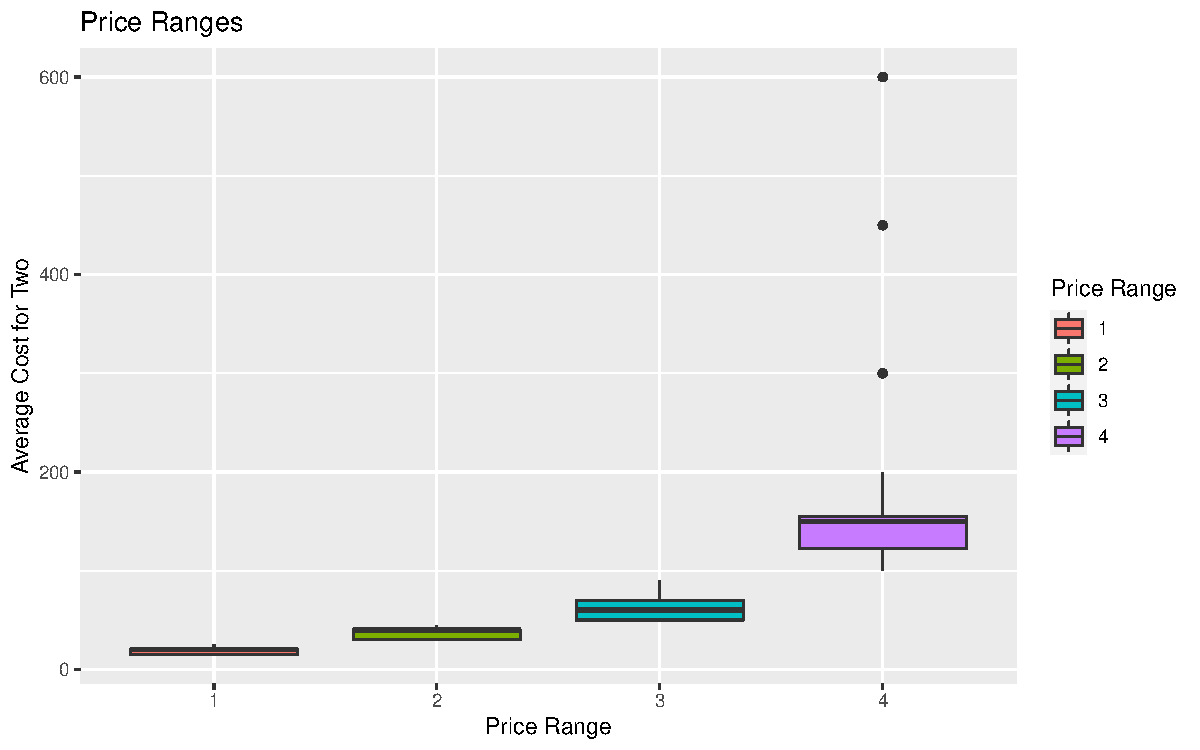
\includegraphics{assignment4_files/figure-latex/price-ranges-1.pdf}
\caption{\label{fig:price-ranges}Price Ranges}
\end{figure}

From Figure \ref{fig:price-ranges} we can see Zomato breaks down price ranges into 4 categories with 4 being the most expensive to 1 being the least expensive.

\begin{table}[!h]

\caption{\label{tab:price-range-table}Price Ranges}
\centering
\begin{tabular}[t]{r|r|r|r|r}
\hline
Price Range & Maximum & Median & Minimum & Range\\
\hline
1 & 25 & 20 & 15 & 10\\
\hline
2 & 45 & 40 & 30 & 15\\
\hline
3 & 90 & 60 & 50 & 40\\
\hline
4 & 600 & 150 & 100 & 500\\
\hline
\end{tabular}
\end{table}

From Table \ref{tab:price-range-table} we can see the range of prices that make up each price category.

\hypertarget{what-the-breakdown-of-price-ranges-of-the-restaurants}{%
\subsection{What the breakdown of price ranges of the restaurants?}\label{what-the-breakdown-of-price-ranges-of-the-restaurants}}

\begin{figure}
\centering
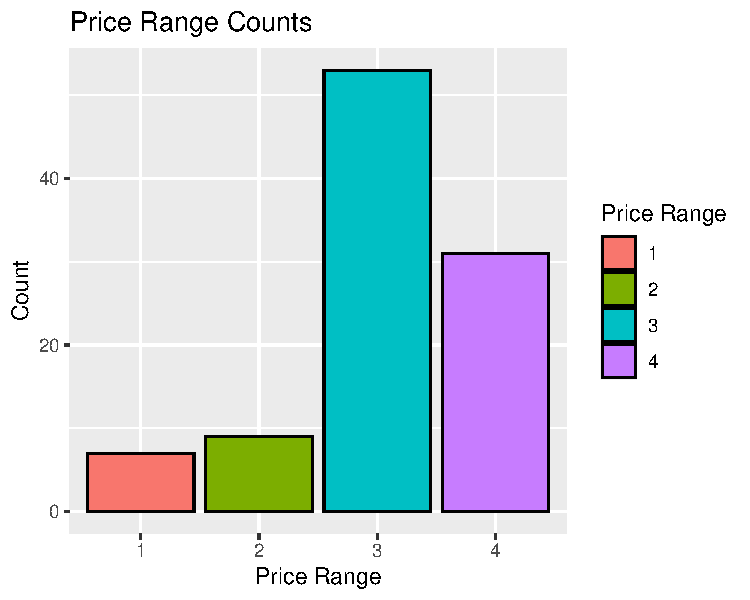
\includegraphics{assignment4_files/figure-latex/price-range-count-1.pdf}
\caption{\label{fig:price-range-count}Price Range Counts}
\end{figure}

From Figure \ref{fig:price-range-count} We can see price range 3 has the most counts. One thing to note however is price range 3 has a range of \$40 compared to 1 and 2 which is \$10 and \$15, respectively. It may be unfair to conclude there is a higher count of more expensive food as the ranges included in the expensive ranges are larger than the lower ones.

\hypertarget{comparing-prices-and-aggregate-ratings}{%
\subsection{Comparing prices and aggregate ratings}\label{comparing-prices-and-aggregate-ratings}}

\begin{figure}
\centering
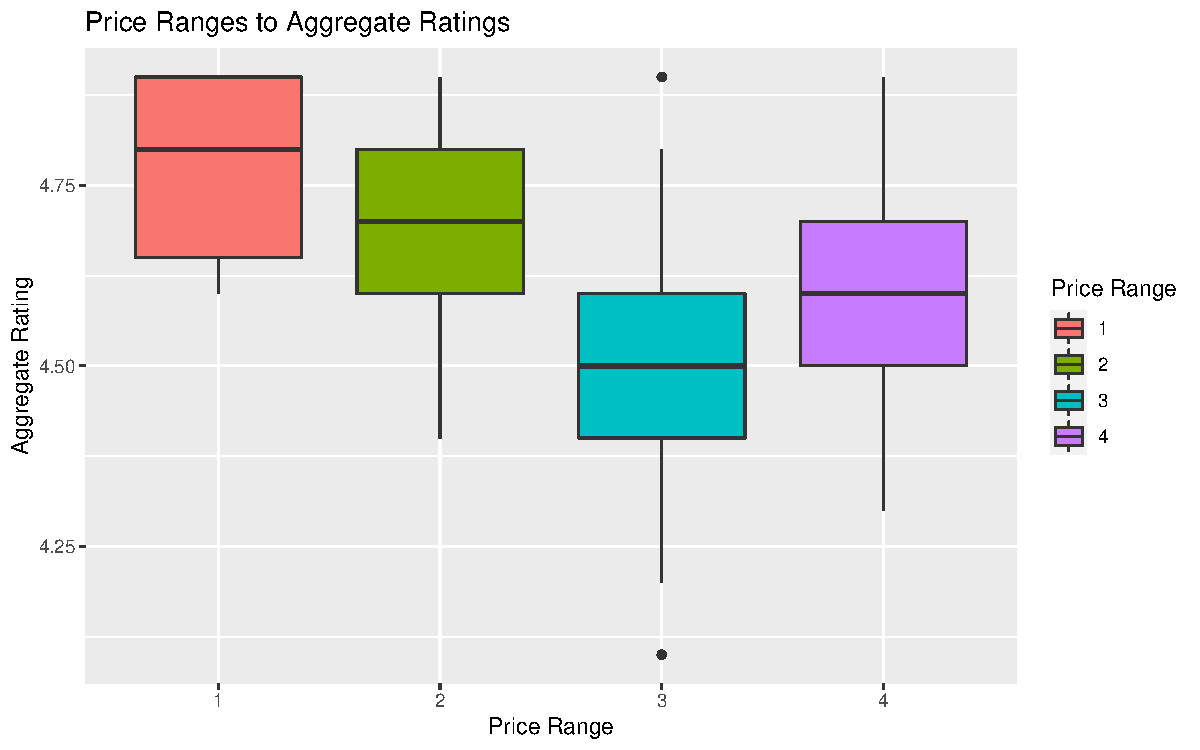
\includegraphics{assignment4_files/figure-latex/price-ratings-1.pdf}
\caption{\label{fig:price-ratings}Price Ranges to Aggregate Ratings}
\end{figure}

From Figure \ref{fig:price-ratings} we can see the median aggregate rating for price range 1 is the highest. In fact, we can see a large amount of lower priced restaurants outranking higher priced restaurants in terms of aggregate ratings.

\hypertarget{is-there-a-relationship-between-prices-and-ratings}{%
\subsection{Is there a relationship between prices and ratings}\label{is-there-a-relationship-between-prices-and-ratings}}

\begin{figure}
\centering
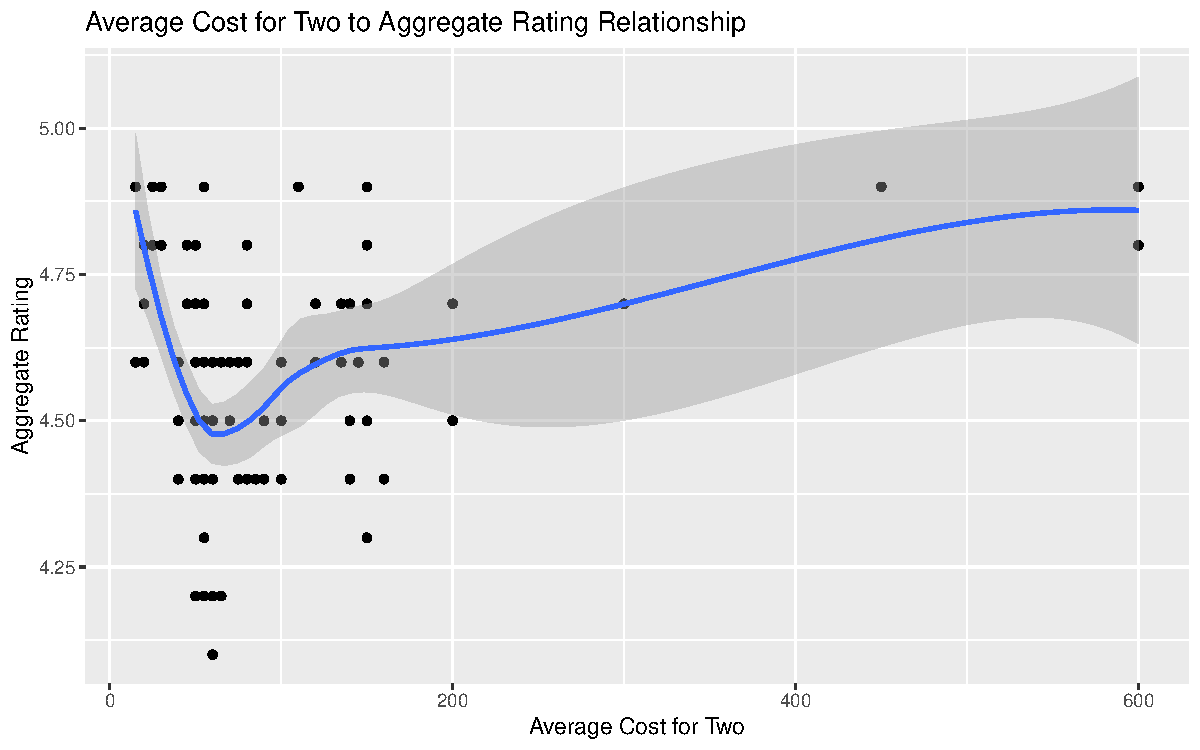
\includegraphics{assignment4_files/figure-latex/cost-rating-relationship-1.pdf}
\caption{\label{fig:cost-rating-relationship}Average Cost for Two to Aggregate Rating Relationship}
\end{figure}

From Figure \ref{fig:cost-rating-relationship} we can see there is not a strong relationship between the average cost for two and the aggregate ratings suggesting there is no relationship between price and food quality. We see a slight upwards trend at the higher price levels. However, this is only based on 5 restaurants with drastically higher prices. We see most of the restaurants fall below the \$200 price point. This might even suggest lower priced restaurants out rank the higher priced restaurants due to the higher count.

\begin{table}[!h]

\caption{\label{tab:rating-ranges}Rating Ranges}
\centering
\begin{tabular}[t]{l|r|r}
\hline
Rating Text & Maximum & Minimum\\
\hline
Excellent & 4.9 & 4.5\\
\hline
Very Good & 4.4 & 4.1\\
\hline
\end{tabular}
\end{table}

Table \ref{tab:rating-ranges} shows range of aggregate ratings that make up each rating levels.

\begin{figure}
\centering
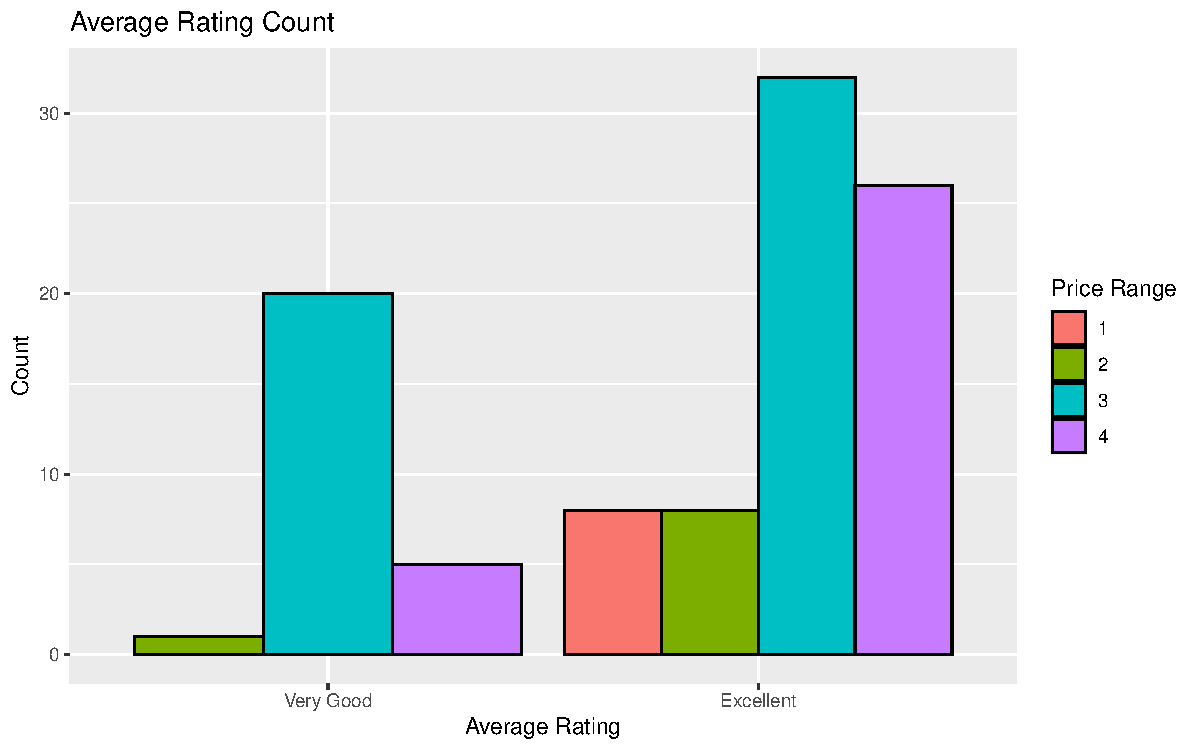
\includegraphics{assignment4_files/figure-latex/rating-count-1.pdf}
\caption{\label{fig:rating-count}Average Rating Count}
\end{figure}

From Figure \ref{fig:rating-count} we can see restaurants in the second and fourth price category all rank in either the very good or excellent category. 3 has the highest count in all categories, however, this may be due to the higher count. We see all price levels have restaurants with high ratings.

\clearpage

\hypertarget{finding-the-very-best-restaurants-of-melbourne}{%
\section{Finding The Very Best Restaurants of Melbourne}\label{finding-the-very-best-restaurants-of-melbourne}}

This section is covering composition and distribution of the very best restaurants in Melbourne-Victoria. In order to find the very best restaurant, this report will filter out 100 restaurants which are listed in \textbf{``Best of Melbourne''} category on Zomato's website. The very best restaurants are described as one which has rating equals to or more than 4.8 out of 5.
After filtered out the dataset, several highest-rated restaurants fill the top list as shown in table \ref{tab:best-restaurant}.

\begin{table}[!h]

\caption{\label{tab:best-restaurant}The Very Best Restaurants in Melbourne According to Zomato Rating}
\centering
\fontsize{8}{10}\selectfont
\begin{tabular}[t]{l|l|l|r|r}
\hline
name & cuisines & locality & price\_for\_two & rating\\
\hline
\cellcolor{pink}{Tipo 00} & \cellcolor{pink}{Italian} & \cellcolor{pink}{CBD} & \cellcolor{pink}{150} & \cellcolor{pink}{4.9}\\
\hline
Le Petit Gateau & French, Desserts, Coffee and Tea & CBD & 30 & 4.9\\
\hline
\cellcolor{pink}{Minamishima} & \cellcolor{pink}{Japanese, Sushi} & \cellcolor{pink}{Richmond} & \cellcolor{pink}{450} & \cellcolor{pink}{4.9}\\
\hline
Dexter & American, BBQ & Preston & 110 & 4.9\\
\hline
\cellcolor{pink}{Vue de monde} & \cellcolor{pink}{Australian, Contemporary} & \cellcolor{pink}{CBD} & \cellcolor{pink}{600} & \cellcolor{pink}{4.9}\\
\hline
Lune Croissanterie & Bakery, French & Fitzroy & 25 & 4.9\\
\hline
\cellcolor{pink}{Beatrix} & \cellcolor{pink}{Coffee and Tea, Bakery} & \cellcolor{pink}{North Melbourne} & \cellcolor{pink}{30} & \cellcolor{pink}{4.9}\\
\hline
Patricia Coffee Brewers & Coffee and Tea & CBD & 15 & 4.9\\
\hline
\cellcolor{pink}{Agathé Pâtisserie} & \cellcolor{pink}{Bakery, Patisserie} & \cellcolor{pink}{South Melbourne Market, South Melbourne} & \cellcolor{pink}{15} & \cellcolor{pink}{4.9}\\
\hline
Hinoki Japanese Pantry & Japanese, Sushi & Fitzroy & 55 & 4.9\\
\hline
\cellcolor{pink}{Humble Rays} & \cellcolor{pink}{Coffee and Tea, Cafe Food, Asian Fusion} & \cellcolor{pink}{Carlton} & \cellcolor{pink}{50} & \cellcolor{pink}{4.8}\\
\hline
Rice Paper Scissors & Asian Fusion, Tapas & CBD & 80 & 4.8\\
\hline
\cellcolor{pink}{Shanklin Cafe} & \cellcolor{pink}{Modern Australian, Coffee and Tea, Cafe Food} & \cellcolor{pink}{Hawthorn} & \cellcolor{pink}{50} & \cellcolor{pink}{4.8}\\
\hline
Bibelot & Desserts, Ice Cream, Cafe Food, Coffee and Tea & South Melbourne & 30 & 4.8\\
\hline
\cellcolor{pink}{Aka Siro} & \cellcolor{pink}{Japanese} & \cellcolor{pink}{Collingwood} & \cellcolor{pink}{80} & \cellcolor{pink}{4.8}\\
\hline
La Belle Miette & Desserts, French, Coffee and Tea & CBD & 20 & 4.8\\
\hline
\cellcolor{pink}{Attica} & \cellcolor{pink}{Australian, Contemporary} & \cellcolor{pink}{Ripponlea} & \cellcolor{pink}{600} & \cellcolor{pink}{4.8}\\
\hline
Shira Nui & Sushi, Japanese & Glen Waverley & 150 & 4.8\\
\hline
\cellcolor{pink}{Punch Lane} & \cellcolor{pink}{Mediterranean, Modern Australian} & \cellcolor{pink}{CBD} & \cellcolor{pink}{150} & \cellcolor{pink}{4.8}\\
\hline
The Proud Peacock & Chinese, Thai, Vietnamese & Mount Waverley & 45 & 4.8\\
\hline
\end{tabular}
\end{table}

From table \ref{tab:best-restaurant} above, there are twelve restaurants which have minimum rating 4.8 out of 5 hence can be described as the very best restaurants in Melbourne. The prices, cuisines and locations in the top list are vary but with some patterns that will be further explored in the following paragraphs.

Regarding the average price and location of the restaurants, figure \ref{fig:maps} shows the map plot of these highest-rated restaurants with their attribute of average food price for two person. The average price for two persons is differentiated by color, while larger circle indicates higher rating (4.9).

It is seen from the figure \ref{fig:maps} that three restaurants are located in CBD, which is not surprising given the nature of CBD as the epicenter of Melbourne. Other restaurants are relatively still located close to CBD like Fitzroy, North Melbourne, Carlton and Hawthorn where eight restaurants base in. One outlier from the list is Shira Nui restaurant, where its location is quite far away from other restaurants in the group. This Japanese-sushi restaurant is located in Glen Waverley suburb which is about one and half hour driving from the CBD.

Furthermore, 4 out of 12 highest-rated restaurants in Melbourne are Japanese-Sushi Restaurants, three are coffee shops, while the rest are french and Australian food restaurants as indicated by figure \ref{fig:map-icon}. This fact support an opinion that ``Japanese food is still growing since UNESCO declared Japanese cuisine to be an Intangible Cultural Heritage in 2013'' \textcite{sushi}.

Furthermore, 4 out of 12 highest-rated restaurants in Melbourne are Japanese-Sushi Restaurants, three are coffee shops, while the rest are french and australian food restaurants as shown by figure \ref{fig:map-icon}.
This fact support an opinion that ``japanese food is still growing since UNESCO declared Japanese cuisine to be an Intangible Cultural Heritage in 2013'' \textcite{sushi}.

\clearpage

\hypertarget{popularity-of-different-cuisines-in-melbourne}{%
\section{Popularity of different cuisines in Melbourne}\label{popularity-of-different-cuisines-in-melbourne}}

In this section we will look at the popularity of different cuisines in Melbourne. The analysis is based on the total votes restaurants serving these cuisine have.

\begin{figure}
\centering
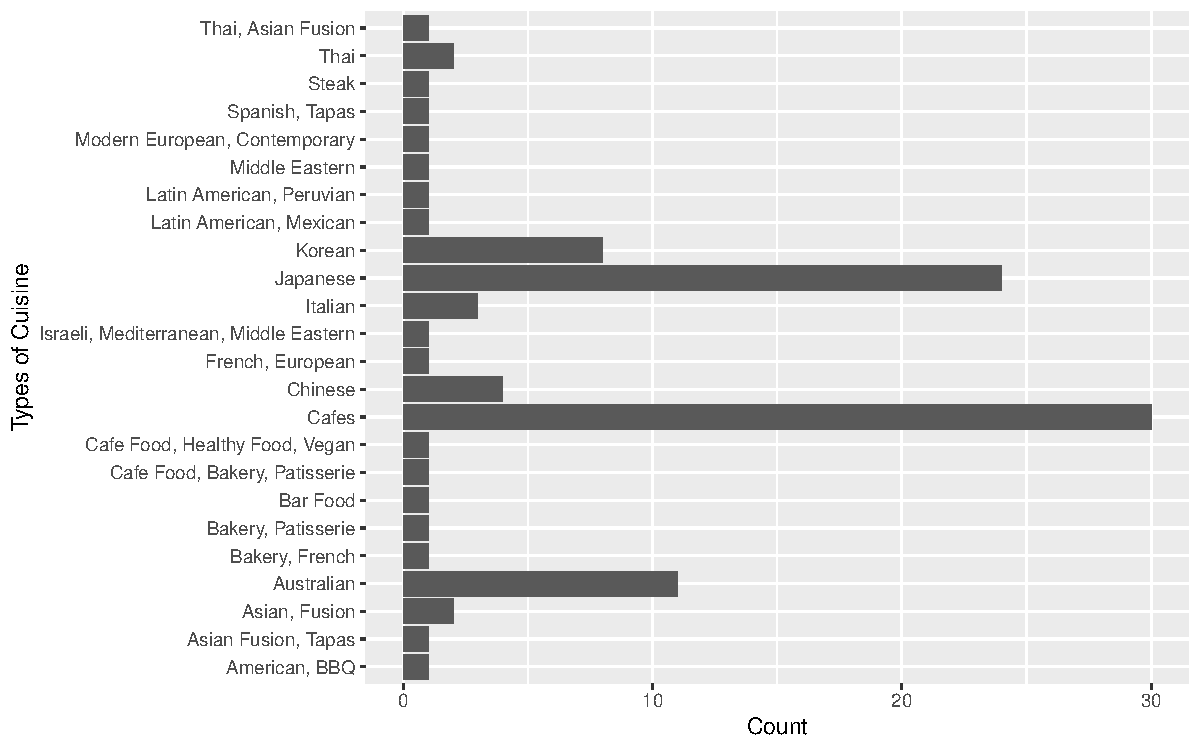
\includegraphics{assignment4_files/figure-latex/Cuisine-Type-1.pdf}
\caption{\label{fig:Cuisine-Type}Number of restaurants for different Cuisines in Melbourne}
\end{figure}

From Figure \ref{fig:Cuisine-Type}, we can see that Japanese cuisine dominates the Melbourne CBD area, with more than 25 restaurants. Korean and Chinese cuisine are second popular with more than 10 restaurants serving these cuisine in the CBD Area. Also we see that CBD has lots of Cafes which can be related to the nature of the area given that CBD is a business hub with a fast pace environment. According to \textcite{Coffee} while many people still rely on a quick takeaway on their way to work or on a break from the office, many cafe's have transformed into restaurants and dining spaces where people can enjoy their hot beverage over a meal or even just to sit down with friends or work colleagues.

\begin{figure}
\centering
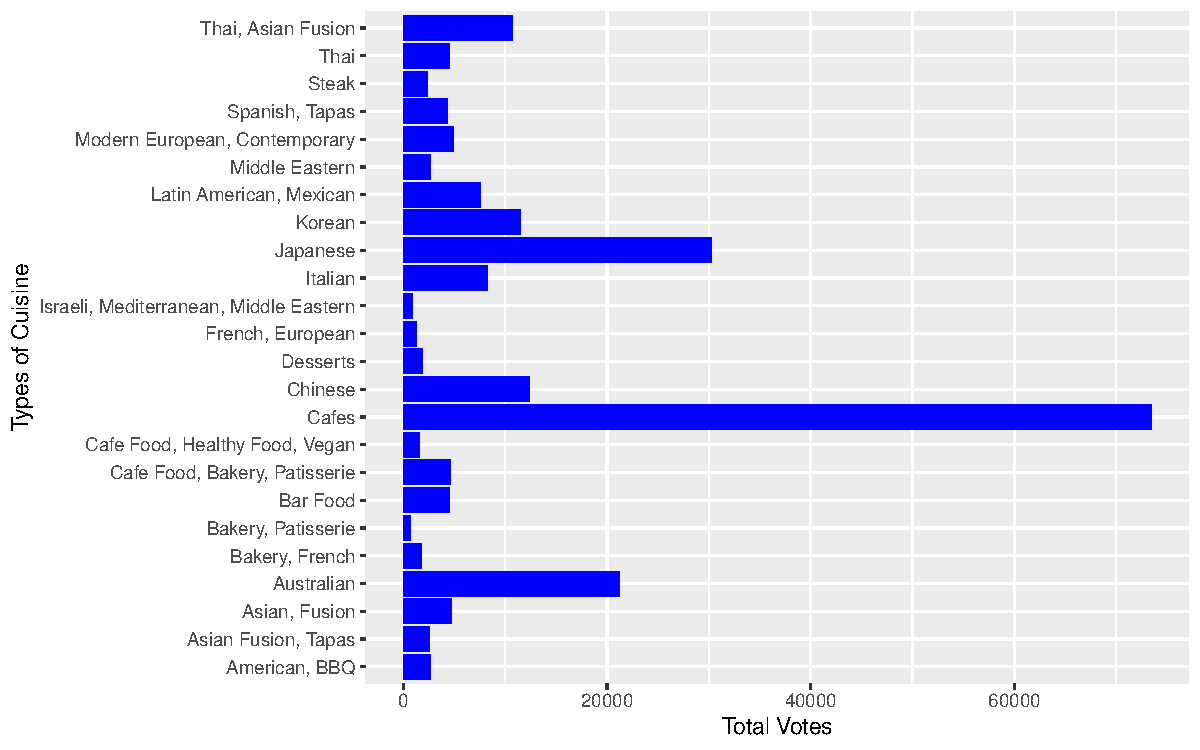
\includegraphics{assignment4_files/figure-latex/Cuisine-Votes-1.pdf}
\caption{\label{fig:Cuisine-Votes}Number of Votes for different Cuisines in Melbourne}
\end{figure}

From Figure \ref{fig:Cuisine-Votes}, we can look at the number of votes for different cuisine types. The popularity of a cuisine can largely be explained the number of votes it gets. Japanese cuisine is very popular. According to \textcite{ATR}, `Chefs and restaurant owners agree diners have become more discerning and want healthy, sustainable and honest food'. The growing popularity has made Japanese restaurants a regular feature on the top restaurants list.

\begin{table}[!h]

\caption{\label{tab:top10-Jap}Top 10 voted Japanese restaurants in Melbourne}
\centering
\begin{tabular}[t]{llrr}
\toprule
name & locality & aggregate\_rating & Total\_Votes\\
\midrule
\cellcolor{gray!6}{Hakata Gensuke Ramen Professionals} & \cellcolor{gray!6}{CBD} & \cellcolor{gray!6}{4.7} & \cellcolor{gray!6}{2337}\\
Purple Peanuts Japanese Cafe & CBD & 4.6 & 2142\\
\cellcolor{gray!6}{Mr. Miyagi} & \cellcolor{gray!6}{Windsor} & \cellcolor{gray!6}{4.7} & \cellcolor{gray!6}{2024}\\
Peko Peko & South Melbourne & 4.6 & 1990\\
\cellcolor{gray!6}{Sakura Kaiten Sushi} & \cellcolor{gray!6}{CBD} & \cellcolor{gray!6}{4.6} & \cellcolor{gray!6}{1856}\\
\addlinespace
Calia & Emporium Melbourne & 4.5 & 1806\\
\cellcolor{gray!6}{Shira Nui} & \cellcolor{gray!6}{Glen Waverley} & \cellcolor{gray!6}{4.8} & \cellcolor{gray!6}{1633}\\
Shoya Nouvelle Wafu Cuisine & CBD & 4.7 & 1514\\
\cellcolor{gray!6}{Kisumé} & \cellcolor{gray!6}{CBD} & \cellcolor{gray!6}{4.5} & \cellcolor{gray!6}{1346}\\
Shou Sumiyaki & CBD & 4.4 & 1263\\
\bottomrule
\end{tabular}
\end{table}

In Table \ref{tab:top10-Jap} we can look at the top ten popular Japanese restaurants with votes count and the locality they are in.

\clearpage

\hypertarget{exploring-gluten-free-foodrestaurants-in-melbourne}{%
\section{Exploring gluten free food/restaurants in Melbourne}\label{exploring-gluten-free-foodrestaurants-in-melbourne}}

In this section we will be looking into restaurants with gluten free food.

We will explore high end restaurants which offer gluten free food.
To look for a good restaurant we will be using aggregate ratings.
Popular restaurants will have more then 500 reviews.
Being realistic, calculating average cost for one person's meal.
Most Instagramable place.

\hypertarget{checking-out-the-category-gluten-free}{%
\subsection{Checking out the category ``Gluten-Free''!}\label{checking-out-the-category-gluten-free}}

For diet conscious people and people with Gluten Allergy.

\hypertarget{selecting-appropriate-variables-and-being-realistic}{%
\subsection{Selecting appropriate variables and being realistic!}\label{selecting-appropriate-variables-and-being-realistic}}

Picking required variables.

\hypertarget{making-an-easy-to-understand-table}{%
\subsection{Making an easy to understand table!}\label{making-an-easy-to-understand-table}}

\begin{table}[!h]

\caption{\label{tab:rest-gluten-free}Top Options}
\centering
\fontsize{8}{10}\selectfont
\begin{tabular}[t]{l|r|r|r|l|l}
\hline
name & avg\_cost\_for\_one & all\_reviews\_count & photo\_count & locality & aggregate\_rating\\
\hline
\cellcolor{gray!6}{Jinda Thai Restaurant} & \cellcolor{gray!6}{40.0} & \cellcolor{gray!6}{1036} & \cellcolor{gray!6}{2478} & \cellcolor{gray!6}{Abbotsford} & \cellcolor{gray!6}{4.7}\\
\hline
Mr Hendricks Cafe & 25.0 & 472 & 1063 & Balwyn & 4.7\\
\hline
\cellcolor{gray!6}{Humble Rays} & \cellcolor{gray!6}{25.0} & \cellcolor{gray!6}{838} & \cellcolor{gray!6}{2566} & \cellcolor{gray!6}{Carlton} & \cellcolor{gray!6}{4.8}\\
\hline
Vertue Coffee Roasters & 25.0 & 465 & 1424 & Carlton & 4.6\\
\hline
\cellcolor{gray!6}{DOC Pizza \& Mozzarella Bar - Carlton} & \cellcolor{gray!6}{35.0} & \cellcolor{gray!6}{926} & \cellcolor{gray!6}{763} & \cellcolor{gray!6}{Carlton} & \cellcolor{gray!6}{4.6}\\
\hline
The Hardware Societe & 30.0 & 2108 & 4229 & CBD & 4.6\\
\hline
\cellcolor{gray!6}{Rice Paper Scissors} & \cellcolor{gray!6}{40.0} & \cellcolor{gray!6}{993} & \cellcolor{gray!6}{2891} & \cellcolor{gray!6}{CBD} & \cellcolor{gray!6}{4.8}\\
\hline
Chin Chin & 67.5 & 3213 & 3270 & CBD & 4.6\\
\hline
\cellcolor{gray!6}{Tipo 00} & \cellcolor{gray!6}{75.0} & \cellcolor{gray!6}{724} & \cellcolor{gray!6}{2129} & \cellcolor{gray!6}{CBD} & \cellcolor{gray!6}{4.9}\\
\hline
Dodee Paidang & 37.5 & 483 & 1007 & CBD & 4.6\\
\hline
\cellcolor{gray!6}{San Telmo} & \cellcolor{gray!6}{60.0} & \cellcolor{gray!6}{767} & \cellcolor{gray!6}{1208} & \cellcolor{gray!6}{CBD} & \cellcolor{gray!6}{4.6}\\
\hline
MoVida Bar De Tapas & 60.0 & 900 & 1160 & CBD & 4.7\\
\hline
\cellcolor{gray!6}{+39 Pizzeria} & \cellcolor{gray!6}{50.0} & \cellcolor{gray!6}{809} & \cellcolor{gray!6}{1185} & \cellcolor{gray!6}{CBD} & \cellcolor{gray!6}{4.6}\\
\hline
Cumulus Inc. & 75.0 & 1125 & 1288 & CBD & 4.7\\
\hline
\cellcolor{gray!6}{Le Petit Gateau} & \cellcolor{gray!6}{15.0} & \cellcolor{gray!6}{352} & \cellcolor{gray!6}{519} & \cellcolor{gray!6}{CBD} & \cellcolor{gray!6}{4.9}\\
\hline
Sakura Kaiten Sushi & 30.0 & 437 & 1111 & CBD & 4.6\\
\hline
\cellcolor{gray!6}{Hakata Gensuke Ramen Professionals} & \cellcolor{gray!6}{25.0} & \cellcolor{gray!6}{845} & \cellcolor{gray!6}{1189} & \cellcolor{gray!6}{CBD} & \cellcolor{gray!6}{4.7}\\
\hline
Vue de monde & 300.0 & 985 & 2755 & CBD & 4.9\\
\hline
\cellcolor{gray!6}{Shoya Nouvelle Wafu Cuisine} & \cellcolor{gray!6}{70.0} & \cellcolor{gray!6}{391} & \cellcolor{gray!6}{1316} & \cellcolor{gray!6}{CBD} & \cellcolor{gray!6}{4.7}\\
\hline
Wonderbao & 10.0 & 773 & 773 & CBD & 4.6\\
\hline
\cellcolor{gray!6}{Brother Baba Budan} & \cellcolor{gray!6}{7.5} & \cellcolor{gray!6}{545} & \cellcolor{gray!6}{446} & \cellcolor{gray!6}{CBD} & \cellcolor{gray!6}{4.6}\\
\hline
Little Rogue & 10.0 & 334 & 671 & CBD & 4.7\\
\hline
\cellcolor{gray!6}{Purple Peanuts Japanese Cafe} & \cellcolor{gray!6}{20.0} & \cellcolor{gray!6}{490} & \cellcolor{gray!6}{661} & \cellcolor{gray!6}{CBD} & \cellcolor{gray!6}{4.6}\\
\hline
Patricia Coffee Brewers & 7.5 & 365 & 292 & CBD & 4.9\\
\hline
\cellcolor{gray!6}{Shimbashi Soba \& Sake Bar} & \cellcolor{gray!6}{27.5} & \cellcolor{gray!6}{368} & \cellcolor{gray!6}{923} & \cellcolor{gray!6}{CBD} & \cellcolor{gray!6}{4.6}\\
\hline
Maha Restaurant & 150.0 & 932 & 1240 & CBD & 4.7\\
\hline
\cellcolor{gray!6}{La Belle Miette} & \cellcolor{gray!6}{10.0} & \cellcolor{gray!6}{477} & \cellcolor{gray!6}{427} & \cellcolor{gray!6}{CBD} & \cellcolor{gray!6}{4.8}\\
\hline
Coda & 72.5 & 562 & 704 & CBD & 4.6\\
\hline
\cellcolor{gray!6}{Punch Lane} & \cellcolor{gray!6}{75.0} & \cellcolor{gray!6}{430} & \cellcolor{gray!6}{862} & \cellcolor{gray!6}{CBD} & \cellcolor{gray!6}{4.8}\\
\hline
Pastuso & 62.5 & 444 & 1048 & CBD & 4.6\\
\hline
\cellcolor{gray!6}{Aka Siro} & \cellcolor{gray!6}{40.0} & \cellcolor{gray!6}{238} & \cellcolor{gray!6}{491} & \cellcolor{gray!6}{Collingwood} & \cellcolor{gray!6}{4.8}\\
\hline
Kenzan Japanese & 80.0 & 263 & 594 & Collins Place & 4.6\\
\hline
\cellcolor{gray!6}{Addict Food \& Coffee} & \cellcolor{gray!6}{20.0} & \cellcolor{gray!6}{570} & \cellcolor{gray!6}{1350} & \cellcolor{gray!6}{Fitzroy} & \cellcolor{gray!6}{4.6}\\
\hline
Naked For Satan & 40.0 & 875 & 885 & Fitzroy & 4.6\\
\hline
\cellcolor{gray!6}{Lune Croissanterie} & \cellcolor{gray!6}{12.5} & \cellcolor{gray!6}{754} & \cellcolor{gray!6}{1831} & \cellcolor{gray!6}{Fitzroy} & \cellcolor{gray!6}{4.9}\\
\hline
Faraday's Cage & 22.5 & 382 & 1096 & Fitzroy & 4.7\\
\hline
\cellcolor{gray!6}{Cutler \& Co} & \cellcolor{gray!6}{100.0} & \cellcolor{gray!6}{570} & \cellcolor{gray!6}{988} & \cellcolor{gray!6}{Fitzroy} & \cellcolor{gray!6}{4.7}\\
\hline
Hell of the North & 67.5 & 418 & 851 & Fitzroy & 4.7\\
\hline
\cellcolor{gray!6}{Hinoki Japanese Pantry} & \cellcolor{gray!6}{27.5} & \cellcolor{gray!6}{274} & \cellcolor{gray!6}{383} & \cellcolor{gray!6}{Fitzroy} & \cellcolor{gray!6}{4.9}\\
\hline
Laksa King & 35.0 & 1304 & 1233 & Flemington & 4.6\\
\hline
\cellcolor{gray!6}{Shira Nui} & \cellcolor{gray!6}{75.0} & \cellcolor{gray!6}{424} & \cellcolor{gray!6}{754} & \cellcolor{gray!6}{Glen Waverley} & \cellcolor{gray!6}{4.8}\\
\hline
Shanklin Cafe & 25.0 & 530 & 1244 & Hawthorn & 4.8\\
\hline
\cellcolor{gray!6}{The Proud Peacock} & \cellcolor{gray!6}{22.5} & \cellcolor{gray!6}{631} & \cellcolor{gray!6}{481} & \cellcolor{gray!6}{Mount Waverley} & \cellcolor{gray!6}{4.8}\\
\hline
Beatrix & 15.0 & 387 & 645 & North Melbourne & 4.9\\
\hline
\cellcolor{gray!6}{Dexter} & \cellcolor{gray!6}{55.0} & \cellcolor{gray!6}{685} & \cellcolor{gray!6}{1498} & \cellcolor{gray!6}{Preston} & \cellcolor{gray!6}{4.9}\\
\hline
Serotonin Eatery & 32.5 & 900 & 1897 & Richmond & 4.6\\
\hline
\cellcolor{gray!6}{Minamishima} & \cellcolor{gray!6}{225.0} & \cellcolor{gray!6}{297} & \cellcolor{gray!6}{1435} & \cellcolor{gray!6}{Richmond} & \cellcolor{gray!6}{4.9}\\
\hline
Attica & 300.0 & 497 & 1852 & Ripponlea & 4.8\\
\hline
\cellcolor{gray!6}{Komeyui} & \cellcolor{gray!6}{75.0} & \cellcolor{gray!6}{249} & \cellcolor{gray!6}{1316} & \cellcolor{gray!6}{South Melbourne} & \cellcolor{gray!6}{4.7}\\
\hline
Peko Peko & 25.0 & 517 & 828 & South Melbourne & 4.6\\
\hline
\cellcolor{gray!6}{Bibelot} & \cellcolor{gray!6}{15.0} & \cellcolor{gray!6}{428} & \cellcolor{gray!6}{1437} & \cellcolor{gray!6}{South Melbourne} & \cellcolor{gray!6}{4.8}\\
\hline
Agathé Pâtisserie & 7.5 & 322 & 634 & South Melbourne Market, South Melbourne & 4.9\\
\hline
\cellcolor{gray!6}{Wagyu Ya} & \cellcolor{gray!6}{75.0} & \cellcolor{gray!6}{395} & \cellcolor{gray!6}{1625} & \cellcolor{gray!6}{South Yarra} & \cellcolor{gray!6}{4.7}\\
\hline
Mr. Miyagi & 40.0 & 908 & 2311 & Windsor & 4.7\\
\hline
\cellcolor{gray!6}{Journeyman} & \cellcolor{gray!6}{27.5} & \cellcolor{gray!6}{839} & \cellcolor{gray!6}{1535} & \cellcolor{gray!6}{Windsor} & \cellcolor{gray!6}{\vphantom{1}4.7}\\
\hline
Journeyman & 27.5 & 839 & 1535 & Windsor & 4.7\\
\hline
\end{tabular}
\end{table}

The Table \ref{tab:rest-gluten-free} shows the name of the restarunts in Melbourne, their locality, number of reviews recieved, aggregate ratings, photo count and how much it costs for one persons gluten free meal on average.

\hypertarget{visualizing-findings}{%
\subsection{Visualizing findings!}\label{visualizing-findings}}

\begin{figure}[H]

{\centering 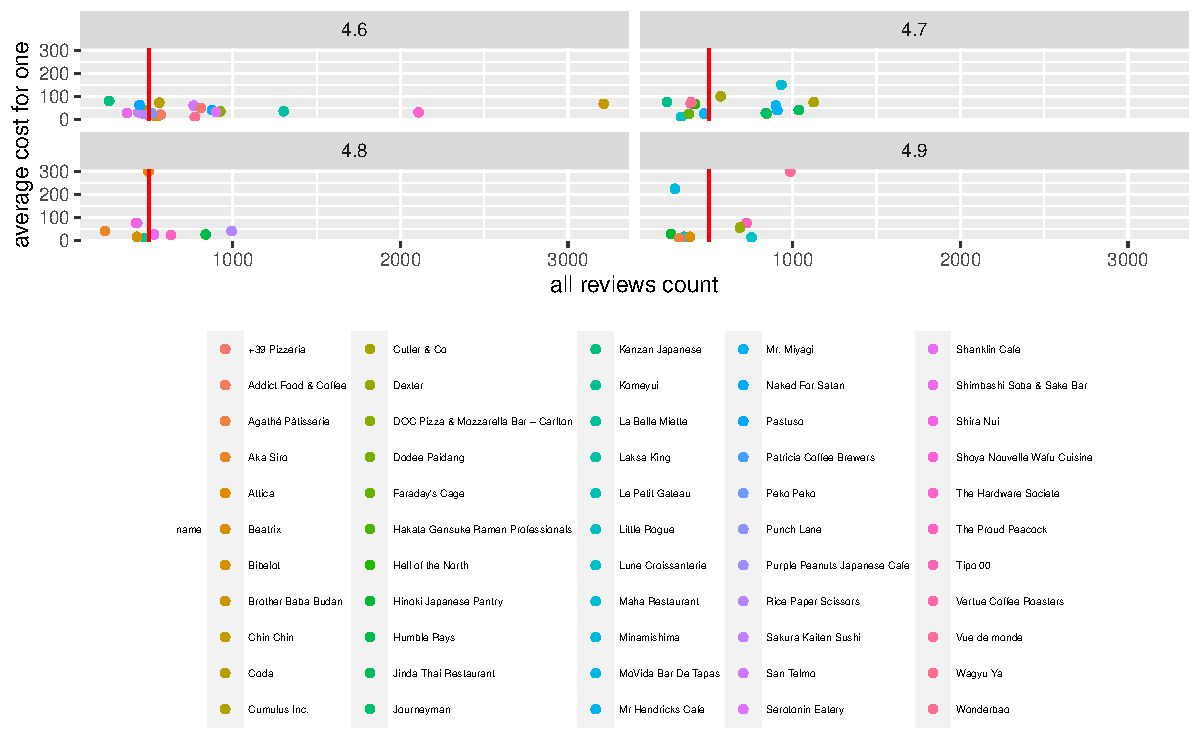
\includegraphics{assignment4_files/figure-latex/review-price-relation-1} 

}

\caption{Worth the money!}\label{fig:review-price-relation}
\end{figure}

The graph Figure \ref{fig:review-price-relation} shows top restaurants in Melbourne, using the category ``gluten free'', with an intercept at 500 reviews count. In the highest rating of 4.9, Lune Croissanterie is the best restaurant with very reasonable average price of 12.50 AUD per person. While, Vue de monde is second on the list with a rating of 4.8 but very pricy at an average cost of 300 AUD.

\begin{figure}[H]

{\centering 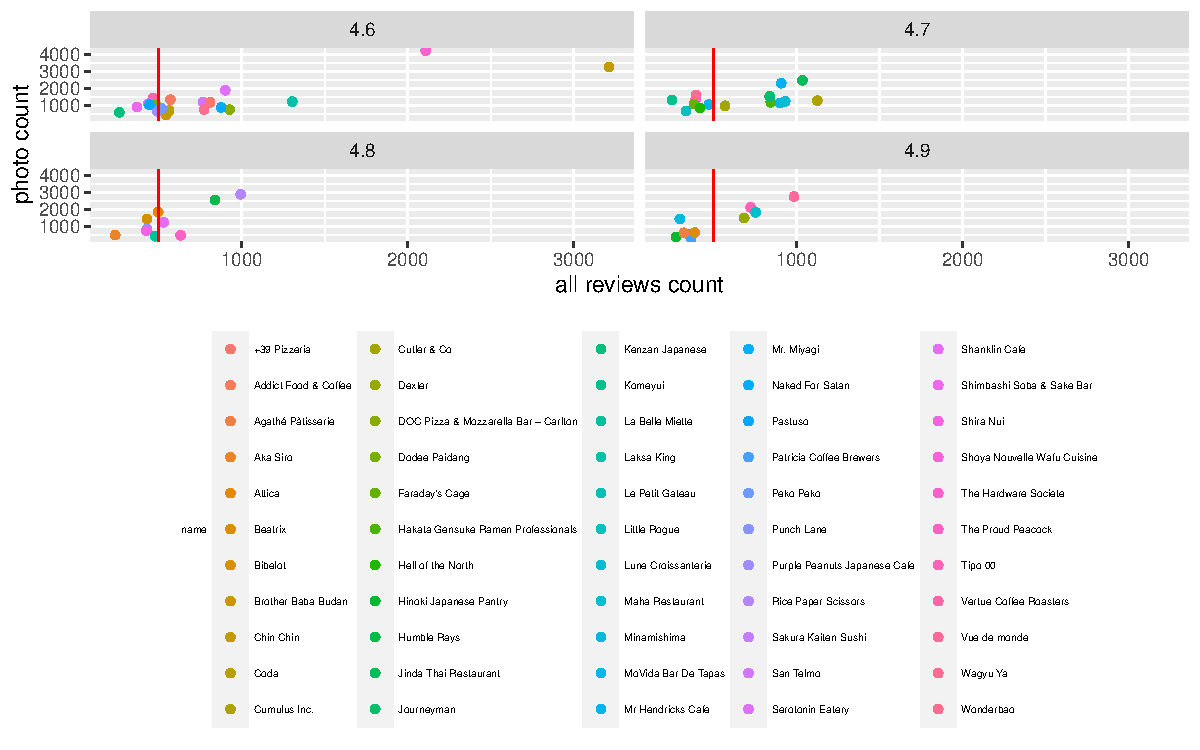
\includegraphics{assignment4_files/figure-latex/instagrammable-plot-1} 

}

\caption{Can I instagram it?}\label{fig:instagrammable-plot}
\end{figure}

The graph Figure \ref{fig:instagrammable-plot} visualizes restaurants with good reviews and potential of each restaurant on how much instagrammable it is. Lune Croissanterie has the best review rating with a high photo count of 1813. While, The Hardware Societe has the highest photo count at 4224, with a good rating of 4.6.

In Table \ref{tab:top10-Jap} we can look at the top 10 popular Japanese restaurants in Melbourne along with their location and rating. `Don-Don' is a very popular Japanese restaurant with 3168 votes. `Shira Nui' is the highest rated restaurant with an aggregated rating of 4.8 out of 5.

The graph Figure \ref{fig:instagrammable-plot} visualizes restaurants with good reviews and potential of each restaurant on how much instagrammable it is. Lune Crissantete has the best review rating with a high photo count of 1813. While, The Hardware Societe has the highest photo count at 4224, with a good rating of 4.6.

\clearpage

\hypertarget{conclusion}{%
\section{Conclusion}\label{conclusion}}

\begin{itemize}
\tightlist
\item
  From this analysis we find there is no real relationship between restaurant prices and quality suggesting expensive food is not better than cheap.
\item
  Melbourne has a strong multicultural cuisines options for people to choose from. Japanese being the most popular has the highest number of restaurants. Popularity of Cafes are also high.
\item
  Most of the very best restaurants in Melbourne is located near CBD.
\item
  Melbourne has quite a few good restaurants which serve gluten free food with a high review count. Most of the the same restaurants have a high photo count as well hence it is instagrammable in my opinion.
\end{itemize}

\clearpage

\printbibliography

\end{document}

